% Static escrow vs Competitive Vickrey auction (§8.4.4).
\documentclass[border=10pt,tikz]{standalone}
\usepackage{tikz}
\usetikzlibrary{arrows.meta,positioning,fit,backgrounds,calc,shapes.geometric}

\definecolor{sand}{HTML}{E9DCC4}
\definecolor{sanddeep}{HTML}{D8C7A6}
\definecolor{ebony}{HTML}{121212}
\definecolor{ink}{HTML}{1B1712}
\definecolor{cobalt}{HTML}{003FB8}
\definecolor{amber}{HTML}{6B4500}
\definecolor{teal}{HTML}{00564C}
\definecolor{paper}{HTML}{FBF7EF}

\begin{document}
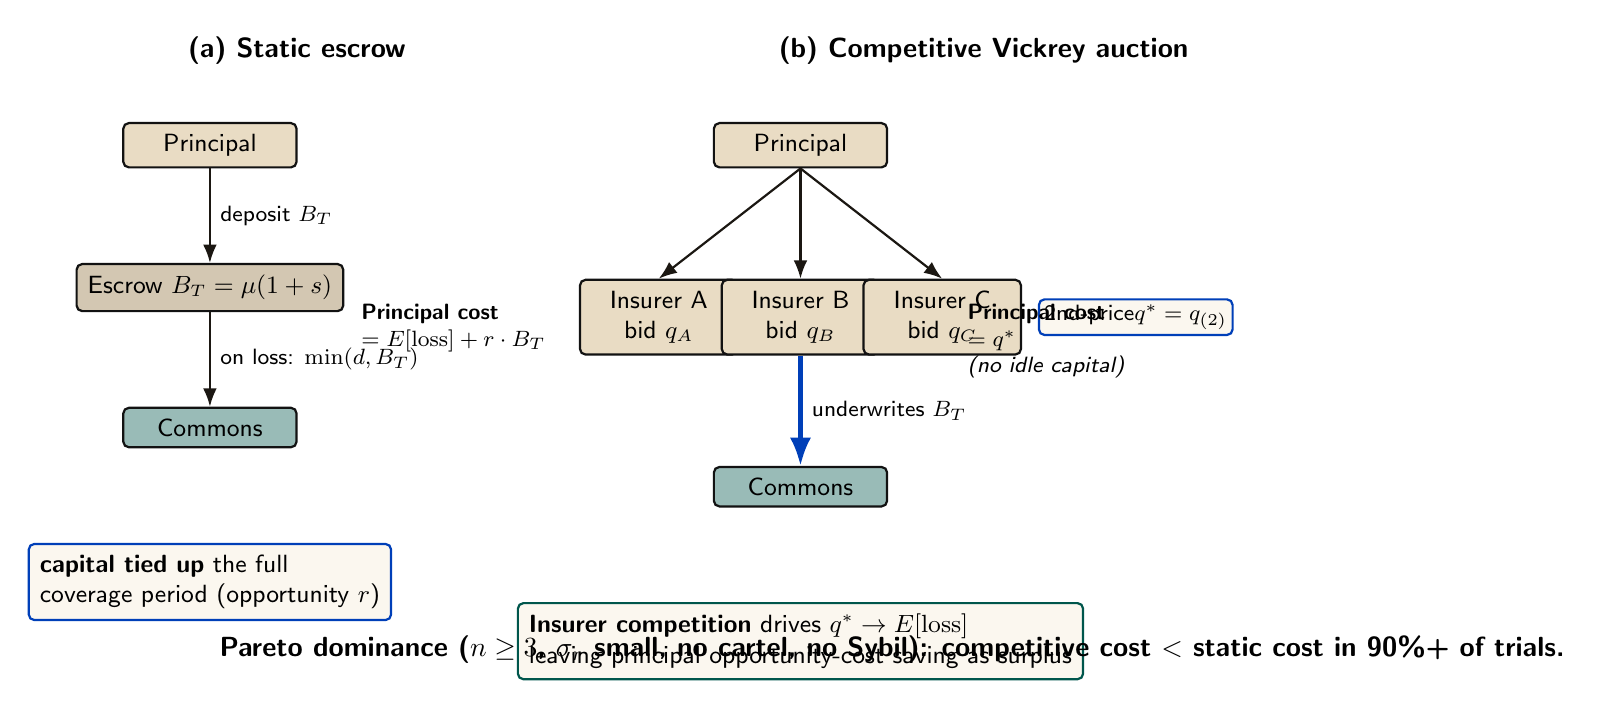
\begin{tikzpicture}[
  font=\sffamily\small,
  actor/.style={draw=ebony,thick,fill=sand,rounded corners=2pt,
                inner sep=4pt,minimum width=22mm,align=center},
  commons/.style={draw=ebony,thick,fill=teal!40,rounded corners=2pt,
                  inner sep=4pt,minimum width=22mm,align=center},
  escrow/.style={draw=ebony,thick,fill=amber!30,rounded corners=2pt,
                 inner sep=4pt,minimum width=22mm,align=center},
  ins/.style={draw=ebony,thick,fill=paper,rounded corners=2pt,inner sep=4pt,
              align=center,minimum width=20mm},
  arr/.style={->,>=Latex,thick,draw=ink},
  flow/.style={->,>=Latex,thick,draw=cobalt},
  panel/.style={draw=ebony,thick,fill=paper,rounded corners=4pt,
                inner sep=8pt},
]

% ===== LEFT PANEL: STATIC =====
\begin{scope}[xshift=0cm]
\node[font=\sffamily\bfseries,anchor=west] at (-0.4,4.6)
  {(a) Static escrow};

\node[actor] (p1) at (0,3.4) {Principal};
\node[escrow,below=12mm of p1] (esc) {Escrow $B_T = \mu(1+s)$};
\node[commons,below=12mm of esc] (c1) {Commons};

\draw[arr] (p1.south) -- node[right,font=\sffamily\footnotesize]
  {deposit $B_T$} (esc.north);
\draw[arr] (esc.south) -- node[right,font=\sffamily\footnotesize]
  {on loss: $\min(d, B_T)$} (c1.north);

\node[align=left,font=\sffamily\footnotesize,
      anchor=north west,xshift=2mm] at (1.6,1.5)
  {{\bfseries Principal cost} \\
   $= \mathbb{E}[\mathrm{loss}] + r \cdot B_T$};

\node[draw=cobalt,thick,fill=paper,rounded corners=2pt,
      inner sep=4pt,below=12mm of c1,align=left,minimum width=42mm]
   {{\bfseries capital tied up} the full\\coverage period (opportunity $r$)};
\end{scope}

% ===== RIGHT PANEL: COMPETITIVE =====
\begin{scope}[xshift=7.5cm]
\node[font=\sffamily\bfseries,anchor=west] at (-0.4,4.6)
  {(b) Competitive Vickrey auction};

\node[actor] (p2) at (0,3.4) {Principal};
\node[ins,fill=sand,below=14mm of p2,xshift=-18mm] (i1) {Insurer A\\bid $q_A$};
\node[ins,fill=sand,below=14mm of p2] (i2) {Insurer B\\bid $q_B$};
\node[ins,fill=sand,below=14mm of p2,xshift=18mm] (i3) {Insurer C\\bid $q_C$};
\node[commons,below=14mm of i2] (c2) {Commons};

% Lowest bid wins; principal pays 2nd-lowest (Vickrey)
\node[draw=cobalt,thick,fill=paper,rounded corners=2pt,inner sep=2pt,
      font=\sffamily\footnotesize,right=2mm of i3]
  (vic) {2nd-price\\$q^* = q_{(2)}$};

\draw[arr] (p2.south) -- (i1.north);
\draw[arr] (p2.south) -- (i2.north);
\draw[arr] (p2.south) -- (i3.north);
\draw[arr,line width=1.6pt,draw=cobalt] (i2.south) --
  node[right,font=\sffamily\footnotesize]
  {underwrites $B_T$} (c2.north);

\node[align=left,font=\sffamily\footnotesize,
      anchor=north west,xshift=2mm] at (1.8,1.5)
  {{\bfseries Principal cost} \\ $= q^*$ \\
   {\itshape (no idle capital)}};

\node[draw=teal,thick,fill=paper,rounded corners=2pt,
      inner sep=4pt,below=12mm of c2,align=left,minimum width=58mm]
   {{\bfseries Insurer competition} drives $q^* \to \mathbb{E}[\mathrm{loss}]$\\
    leaving principal opportunity-cost saving as surplus};
\end{scope}

\node[font=\sffamily\bfseries,anchor=west] at (0,-3.0)
  {Pareto dominance ($n \geq 3$, $\sigma_r$ small, no cartel, no Sybil):
   competitive cost $<$ static cost in 90\%+ of trials.};

\end{tikzpicture}
\end{document}
